% Chapter 5

\chapter{Software Module Implementation}
\label{Chapter 5}
\lhead{}

% use \verb|Samp_Dist_Corr| notation for underscores
%\documentclass{article}
%\texttt{Samp\_Dist\_Corr}
%\verb|Samp_Dist_Corr|
%\texttt{Samp\char`_Dist\char`_Corr}

\section{Overview}
This chapter explains how each of the three modules discussed in the previous chapter are implemented in software. First, Wisard\_Browser\_Module is discussed. Cmd\_Generator\_Module is discussed next, followed by Validation\_Module. Validation\_Module is discussed last because it has the broadest impact on the other modules and the system as a whole. 

\section{WiSARD Browser}
Wisard\_Browser\_Module is a collection of software components which address four major objectives.

\begin{itemize}
	\item Allow a user to specify WiSARD search parameters through a user interface
	\item Search the WiSARDNet PostgreSQLdatabase for WSN state information
	\item Produce a set of WiSARD data objects matching the search criteria specified by the user
	\item The module should integrate with the existing WiSARDNet software
\end{itemize}

% flow of execution - wisard browser module
Figure \ref{fig:wisard_browser_flow} shows the flow of execution for this module. Each procedure shown is described in this chapter.

\begin{figure}[H]
	\centering
	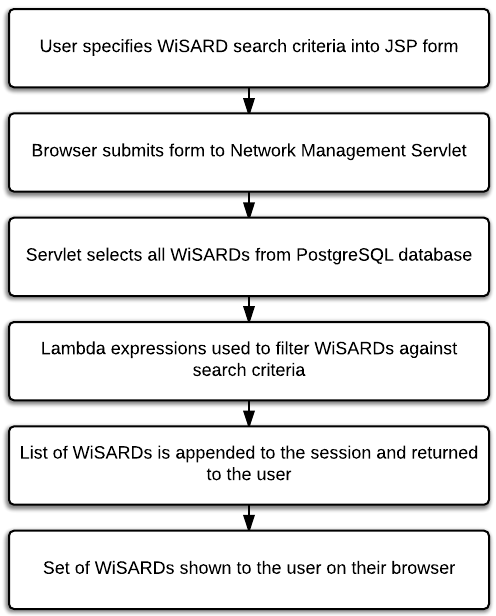
\includegraphics[width=0.6\textwidth]{figures/flow_diagram_wisard_browser.png}
	\caption{Flow of actions performed by Wisard\_Browser\_Module}
	\label{fig:wisard_browser_flow}
\end{figure}

\subsection{Obtaining the User's Search Criteria}
A user of this system needs an interface that allows them to send and receive information to Wisard\_Browser\_Module, Cmd\_Generation\_Module, and Validation\_Module. To create this interface, JSP (JavaServer Pages) and Java servlet technologies are both used. A JSP page presents information to a user through a web browser and gathers user input necessary for back-end operations. The JSP page sends information to and from a servlet called NetworkManagementServlet, which is a java class that implements methods that respond to Get and Post requests from a web browser. Because NetworkManagementServlet is an instance of a Java class, it has the ability to interact with instances of other classes. JSP/servlet interaction is the communication pipeline which allows the user to interact with these three software modules. Figure \ref{fig:jsp_interaction} illustrates how NetworkManagementServlet is used to send and receive information between a user's browser to the appropriate software module. 

\begin{figure}[H]
	\centering
	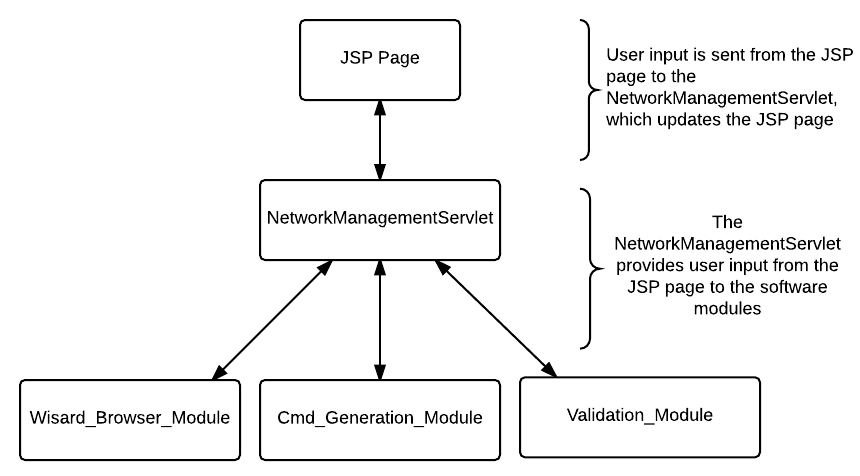
\includegraphics[width=\textwidth]{figures/jsp_interaction.png}
	\caption{NetworkManagementServlet relays information between the user interface and Wisard\_Browser\_Module, Cmd\_Generation\_Module, and Validation\_Module.}
	\label{fig:jsp_interaction}
\end{figure} 

A JSP web page provides a simple interface for the user to populate an HTML form. The attributes that can be used to select a set of WiSARDs are (\ref{fig:jsp_ui_select})

\begin{itemize}
	\item WiSARD Network ID
	\item Device Serial ID
	\item Garden Site
	\item Associated Experiment
	\item SP type
	\item Transducer type
	\item WiSARD role
	\item Deployment Type
\end{itemize} 

\begin{figure}[H]
	\centering
	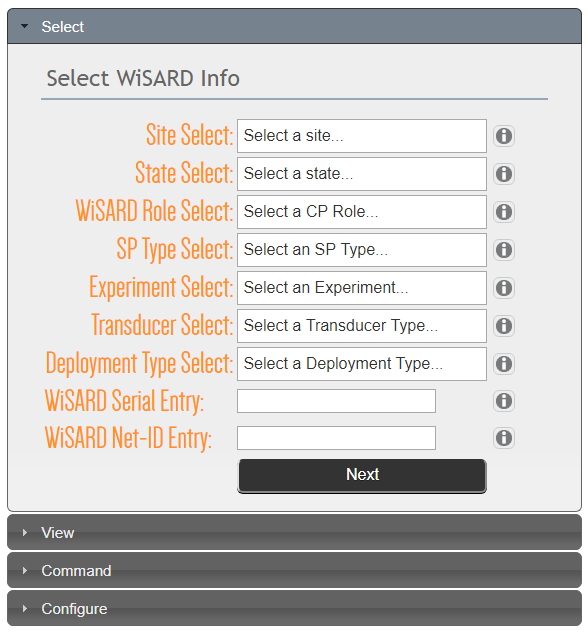
\includegraphics[width=0.6\textwidth]{figures/jsp_ui_select.png}
	\caption{A screen capture of the user interface page where a user specifies WiSARD search criteria}
	\label{fig:jsp_ui_select}
\end{figure}

These attributes are are static or dynamic pieces of information that together represent the current state of the WSN nodes. Traditionally, this information can be obtained from a database query that can be written into a function or a method. Researchers and other users of WiSARDNet often have changing or new experiment requirements. It is important for the this software to be flexible and support changes to the WiSARDs and their configuration information. For example, if new WiSARD features are added, resulting in new fields in a database table or entirely new tables, the new features should not prompt extensive modification of the existing code. A new field or table would simply translate into new member variables in the WiSARD class. 

To implement the querying functionality for Wisard\_Browser\_Module that was discussed in 4.3.1.1, there were two possible design alternatives for the filtration that would result in a list of WiSARDs: PostgreSQL or Wisard\_Browser\_Module application code. PostgreSQL supports a wide variety of query features that enable sophisticated data processing and filtration of queried data sets. If achieving the fastest possible query speed was of great importance for this module, then all of the searching and filtration of WiSARDs from the user's search criteria should be handled by complex PostgreSQL queries. While query time is important, the benefits that can be gained at the sacrifice of processing speed make the other alternative desirable. Chapter 2 briefly explained some of the ways in which modern software development techniques such as behavioral parameterization can add functionality to software. For Wisard\_Browser\_Module, a functional data processing approach allows for development flexibility at the expense of performance overhead. This does not impact the performance of the system in a significant way because the amount of WiSARD deployment configuration information compared to the total amount of data stored in the database is trivial.

WiSARD objects translate from fields in database tables to software entities through the use of intermediate Java classes. A Java class with member variables that correspond to the different attributes that define a WiSARD's configuration, and methods to translate higher-level queries into database queries and results provides a foundation for objects to be created and passed from module to module. To achieve the desired flexibility, Wisard\_Broswer\_Module performs a single fetch to the database and retrieves all of the state information for all of the WiSARDs. It then formats the information from the query into member variables of WiSARD objects before adding them to a list data structure. All of this functionality is built into WiSARD class methods.

Once NetworkManagementServlet has obtained a list of all WiSARD objects, it then filters that list against the attributes which the user specified in his/her form submission. Utilizing functional data processing techniques supported by lambda expressions in Java 8, obtaining a list that matches a user's search criteria is simple and flexible. Below is an example of the way in which lambda expressions are used in this software to produce powerful results with a very small amount of code.

\begin{lstlisting}
return wisards.where((Wisard w) -> ''Arboretum''.equals(w.getSite()));
\end{lstlisting}

This statement returns an ArrayList named \verb|wisards| that contains WiSARD objects. The \verb|where()| method iterates over every entry in the ArrayList and only returns those not filtered out against the logic in the lambda expression. The lambda expression in this example compares the WiSARD site against a string containing the site name \verb|Arboretum|. Any WiSARD in the ArrayList that does not have \verb|Arboretum| as its site name will not be added to the returned ArrayList.

With one line of code, a data structure of WiSARD objects can  be filtered based on its member variables that would otherwise have required a specific database query. Additionally, values can be added to the same expression to create more complex data filtration without requiring that the underlying functionality be altered. This functionality provides a quick and versatile way to support changing project requirements for managing networks of WiSARDs without being restricted by specific database queries.

When a list of WiSARDs has been filtered to match a user's search, NetworkManagementServlet appends it to the session as a variable where it is accessible to the JSP page at the user's browser. The JSP page displays the WiSARDs and their deployment information for the user. From this point a user can decide to continue with reconfiguring the WiSARDs that this search has returned, or return to the form and specify a different set of WiSARDs. Should the user choose to continue on with the set of WiSARDs they have selected, the data structure is accessible within the browser session, ready to send to Command\_Generation\_Module.

\section{Command Generation}
Cmd\_Generation\_Module and Wisard\_Browser\_Module, are similar in that they both rely on user input being sent from the user interface to NetworkManagementServlet. The user will utilize the same JSP page's user interface as Wisard\_Browser\_Module to specify the change he/she would like to apply to the selected WiSARDs (Figure \ref{fig:jsp_ui_cmd}). Each menu option corresponds to a different configuration change that can be selected.\\

\begin{figure}[H]
	\centering
	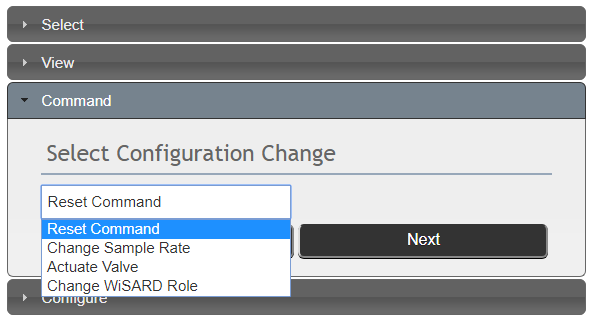
\includegraphics[width=0.6\textwidth]{figures/jsp_ui_cmd.png}
	\caption{A screen capture of the user interface where configurations can be specified}
	\label{fig:jsp_ui_cmd}
\end{figure}

Once a user has selected an option, the process of synthesizing the appropriate commands can proceed. Figure \ref{fig:flow_cmd_generator} shows the flow of execution for this module. Each procedure shown in the diagram is described in this section.\\

% flow of execution, cmd module
\begin{figure}[H]
	\centering
	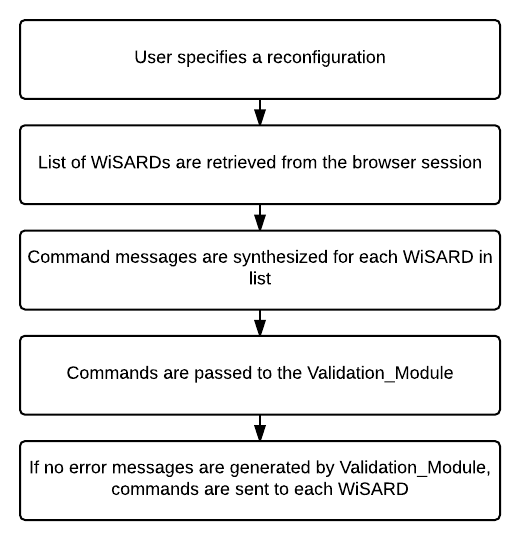
\includegraphics[width=0.6\textwidth]{figures/flow_diagram_cmd_module.png}
	\caption{A flow diagram showing each action Cmd\_Generation\_Module makes}
	\label{fig:flow_cmd_generator}
\end{figure}

To perform a reconfiguration in WiSARDNet, a specific command is generated and sent to each WiSARD that the change will affect. A command in the WiSARDNet communication protocol consists of multiple components. A hub address and a destination address describe which WSN the command should go to, and which WiSARD in the WSN that the command is intended for.

These potential reconfigurations include a soft reset on the device, updating a sampling rate, changing a software role or ID, or actuating a water valve. The list of commands that are possible with a WiSARD continues to grow with each new experiment and feature that WiSARDNet supports. For this reason, the of the design of command synthesis is implemented in a way that provides flexibility for future developments. In WiSARDNet, a command consists of a payload, an expiration, and a checksum. The payload is the byte stream which contains the command and its parameters the WiSARD will interpret and execute. The expiration is a value which the sender sets to prevent out of date commands from being executed. For example, if a command for some reason takes an hour to traverse the network, it may no longer be relevant and should not be executed. The checksum allows the destination WiSARD to verify that it received the command correctly. Each of these command components are encapsulated within a command class named NetManagementCommand.

The class definition for NetManagementCommand provides the member variables and methods for every command type. However, certain commands need additional parameters which aren't provided in NetManagementCommand's class definition. For this reason, a specific class is defined for each command type. Each command class uses inheritance to extend the member variables and methods provided by NetManagementCommand. Table \ref{tab:commands} lists each of the command classes that have been implemented and the reconfiguration change that they make.\\

%%% LIST COMMAND CLASSES HERE IN A TABLE %%%
\begin{table}[H]
	\centering
	\renewcommand{\arraystretch}{1.1}
	\begin{tabular}{|p{3cm}|p{11cm}|}
	\hline
	Command Class & Operation\\
	\hline
	SetSamplingRate & Adjusts the sampling rate of all transducers of a given type on a WiSARD\\
	\hline
	ResetCommand & Performs a soft reset on a WiSARD\\
	\hline
	ActuateValve & Actuates a latching solenoid water valve to an open or closed state\\
	\hline
	ChangeRole & Changes the software role of a WiSARD \\
	\hline
	\end{tabular}
	\caption{A list of each of the command classes that have been implemented}
	\label{tab:commands}
\end{table}

To perform a reconfiguration, a command object is instantiated from the command class definition that corresponds to the user's specified configuration. The change that the user specifies will be enacted for all of the WiSARDs in the list that was added to the session by NetworkManagementServlet. Cmd\_Generation\_Module loops through each WiSARD and chooses the correct command parameters to include in the payload. Once the command objects have been successfully generated they are sent to Validation\_Module in a data structure, similar to the way that Wisard\_Browser\_Module provides the WiSARD list to Cmd\_Generation\_Module.


% 5.3 Command Validation
% 5.3.1 overview of validation
% - types of validation, UAC and safety
% 5.3.2 Permissions and UAC
% - Describe the design of permissions in the database
% - Remember that this will only be for WiSARDs now but state that the permission resource table could be expanded to anything 
% 5.3.3 Safety Validation
% - Describe use cases and how different commands require different checks
% - Describe design of commands with own validation logic so can be flexible
% - Describe that the validate method is given the database wisard and so all relevant parameters can be obtained through normal database relations?

\section{Validation}
Before commands can be sent out to reconfigure WiSARDs, there are two sets of checks which the commands must pass. First, Validation\_Module confirms that the user that submitted the commands has appropriate permissions to reconfigure the selected WiSARD nodes. Second, the module assess the commands for their impact on the system, and ensures that none of the changes will cause a WiSARD to misbehave. WiSARDs may have hardware that is shared between multiple experiments, and reconfiguring that WiSARD could have adverse effects on one or more experiments. The procedures that this module performs are shown in Figure \ref{fig:flow_validation_module}. Each of these procedures is described in this section.\\

% flow of execution, validation module
\begin{figure}[H]
	\centering
	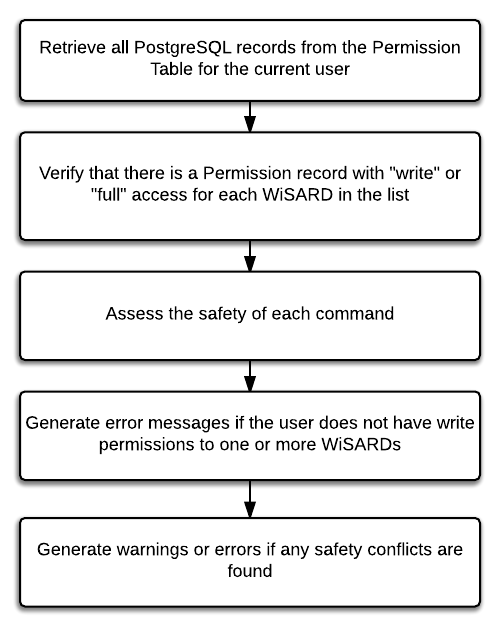
\includegraphics[width=0.6\textwidth]{figures/flow_diagram_validation_module.png}
	\caption{A flow diagram showing each action of Validation\_Module}
	\label{fig:flow_validation_module}
\end{figure}

\subsection{Permissions and User Access Control}
The PostgreSQL database schema prior to this thesis had certain tables which could have been used for user access control, but the schema was not robust. To implement user access control in a flexible way, a better approach was needed. Two core abstractions of the existing database schema are used to design the permissions system for WiSARDNet. The first abstraction is that anyone to whom a permission might be granted is considered a permission entity. The second abstraction is that anything which would need its access restricted is to be considered a permission resource. After applying these two abstractions to the database, the Person and Organization tables are defined as permission entities. Likewise, the Deployment, Site, and Experiment tables are defined as deployment resources. With these two abstractions, granting permission simply becomes a mapping between a permission entity and a permission resource with a value designating the level of access the entity has to the resource.

Two access levels are used to denote permissions to resources: read and write. Table \ref{tab:permissions} describes what each permission level allows. Note that an entity with write access can override changes made by other entities with write access, but a warning message is generated to inform the user of the scenario. In this case, the user should proceed at their own discretion, and the permissions should be granted by an administrator with this in mind. In the greater context of the user access control paradigm, additional access levels could be added to allow delete privileges. Even though that use case doesn't directly correlate to the reconfiguration software, the paradigm still supports that feature for other applications. These two permission levels are sufficient to regulate how users  interact with the WiSARDs. 

This approach to user access control also provides a flexible way to manage other hardware or software resources which might be incorporated into WiSARDNet in the future. If a new type of resource is added to the system which is described by a new table, then adding a foreign key constraint from PermissionResource to the new table is all that is needed for a record in Permission to grant permissions to that new PermissionResource.\\

%\begin{table}[H]
%	\centering
%	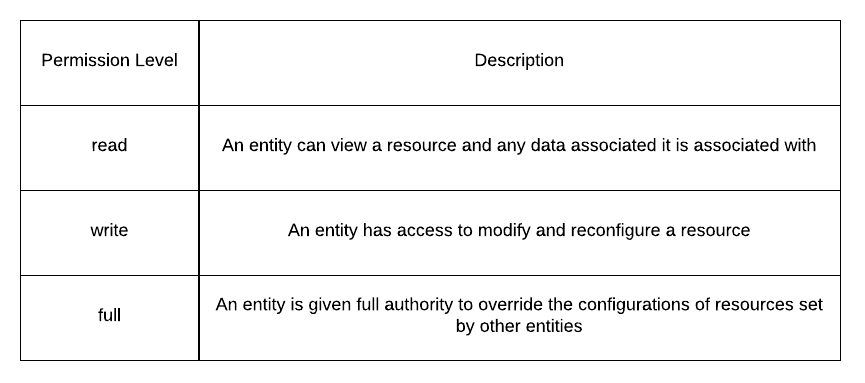
\includegraphics[width=\textwidth]{figures/permission_table.png}
%	\caption{A description of each access level an entity can be granted to a resource}
%	\label{tab:permissions}
%\end{table}

\begin{table}[H]
	\centering
	\renewcommand{\arraystretch}{1.1}
	\begin{tabular}{|p{3cm}|p{11cm}|}
	\hline
	Permission Level & Description\\
	\hline
	read & An entity can view a resource and all information regarding its deployment configuration \\
	\hline
	write & An entity has access to  modify and reconfigure a resource\\
	\hline
	\end{tabular}
	\caption{A description of each access level an entity can be granted to a resource}
	\label{tab:permissions}
\end{table}

To implement user access control with this approach, three tables were added to the database. First, a table called PermissionEntity was created to reference the Person and Organization tables. Next, a table called PermissionResource was created to reference the Deployment, Experiment, and Site tables. Lastly, a table called Permission was created with foreign key constraints that reference the PermissionEntity and PermissionResource primary keys. Each record in Permission specifies an access level value that a PermissionEntity record has to a PermissionResource record. Figure \ref{fig:uac_simplified} shows these tables and their foreign key constraints. Each foreign key constraint references the primary key of the table that the arrow points to. The unnamed table on the right shows how the schema can be used to manage new resources in the future.

\begin{figure}[H]
	\centering
	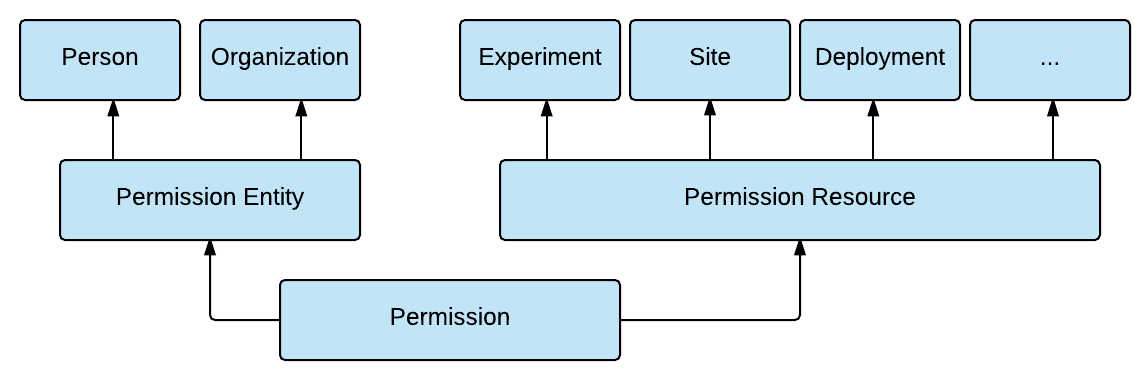
\includegraphics[width=\textwidth]{figures/uac_simplified.png}
	\caption{A diagram that shows how the three new Permission tables are used to create a user access control schema}
	\label{fig:uac_simplified}
\end{figure}

When Validation\_Module receives a data structure of command objects from the command generation module, the software in Validation\_Module first checks that there are no user access violations in any of the commands. This is done by iterating over each command object and performing a lookup to the permission table. The objective is to gather all of the Permission records whose permission entity matches the user that created the commands, and verify that a permission resource with write access is present, for the WiSARD in question. If the user is found to have insufficient permissions to execute a command, an error message is generated and added to a queue of messages that is displayed once Validation\_Module has iterated over every command. All commands with insufficient permissions are rejected, and will not be sent to the WiSARDs.

The validation logic for the reconfiguration software currently grants permissions to WiSARDs. However, the database schema supports a more granular level of detail. A record in the permission resource table could reference the deployment of a device, meaning that access to a WiSARD could be restricted down to individual transducers. 

\subsection{Safety Validation}
 If all of the commands pass the user access permission checks, then the module performs a configuration safety test on each command. The difficulty of the safety check comes from the different types of commands that can be executed, and the diversity of experiments and their needs. It is for this reason that the command class was designed such that each command type will implement its own safety logic. This way, when a new command is developed, the designer can build in a method which will perform a safety check within the context of that method. Figure \ref{fig:cmd_classes} shows the structure of these command classes and how they inherit and override behaviors.
 
\begin{figure}[H]
	\centering
	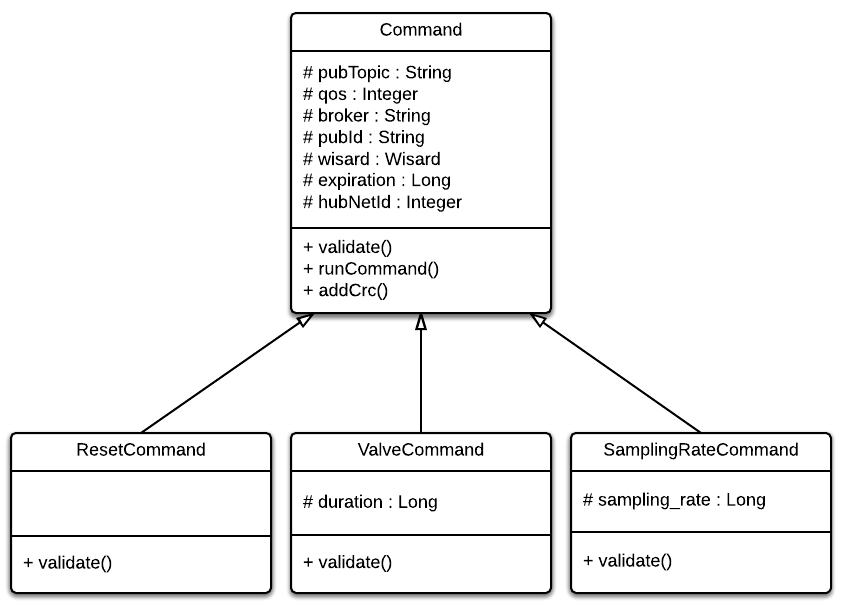
\includegraphics[width=\textwidth]{figures/command_class_diagram.png}
	\caption{A class diagram showing how new commands inherit from their parent class, yet implement their own validate method}
	\label{fig:cmd_classes}
\end{figure}
 
 A practical example of a safety validation method would be a case where a particular command is designed to increase the sampling rate of a particular transducer type on a WiSARD. Here, an appropriate safety check would ensure that the new sampling rate is a reasonable value. For example, if the user enters a non-numeric value, a negative value, or a value corresponding to a sampling rate which the WiSARDs cannot physically perform, those should result in a failed safety check where the command is rejected. Another example is a command to reconfigure a WiSARD that one or more experiments are using. If a configuration change is specified for a WiSARD associated with an experiment, a warning message is generated and added to a queue that is shown to the user. In any scenario where multiple users have write access to a WiSARD, the command is not rejected but the user will be warned of the conflict through a message. 

\section{Summary}
Each of the three software modules developed for this thesis serves a distinct role in enabling WiSARD reconfiguration. Wisard\_Browser\_Module is a flexible module that enables users to search for and select a group of WiSARDs based on a range of network state information. Cmd\_Generation\_Module enables a user to select a change he/she would like to make to the set of selected WiSARDs, and automatically generate the commands necessary to implement those changes. Validation\_Module performs user access control and network safety checks to ensure that all reconfigurations are made in a way that eliminates conflicts. The design and implementation of these three modules provides great flexibility to developers who will work on the WiSARDNet platform in the future.
